\begin{figure}[H]
  \centering
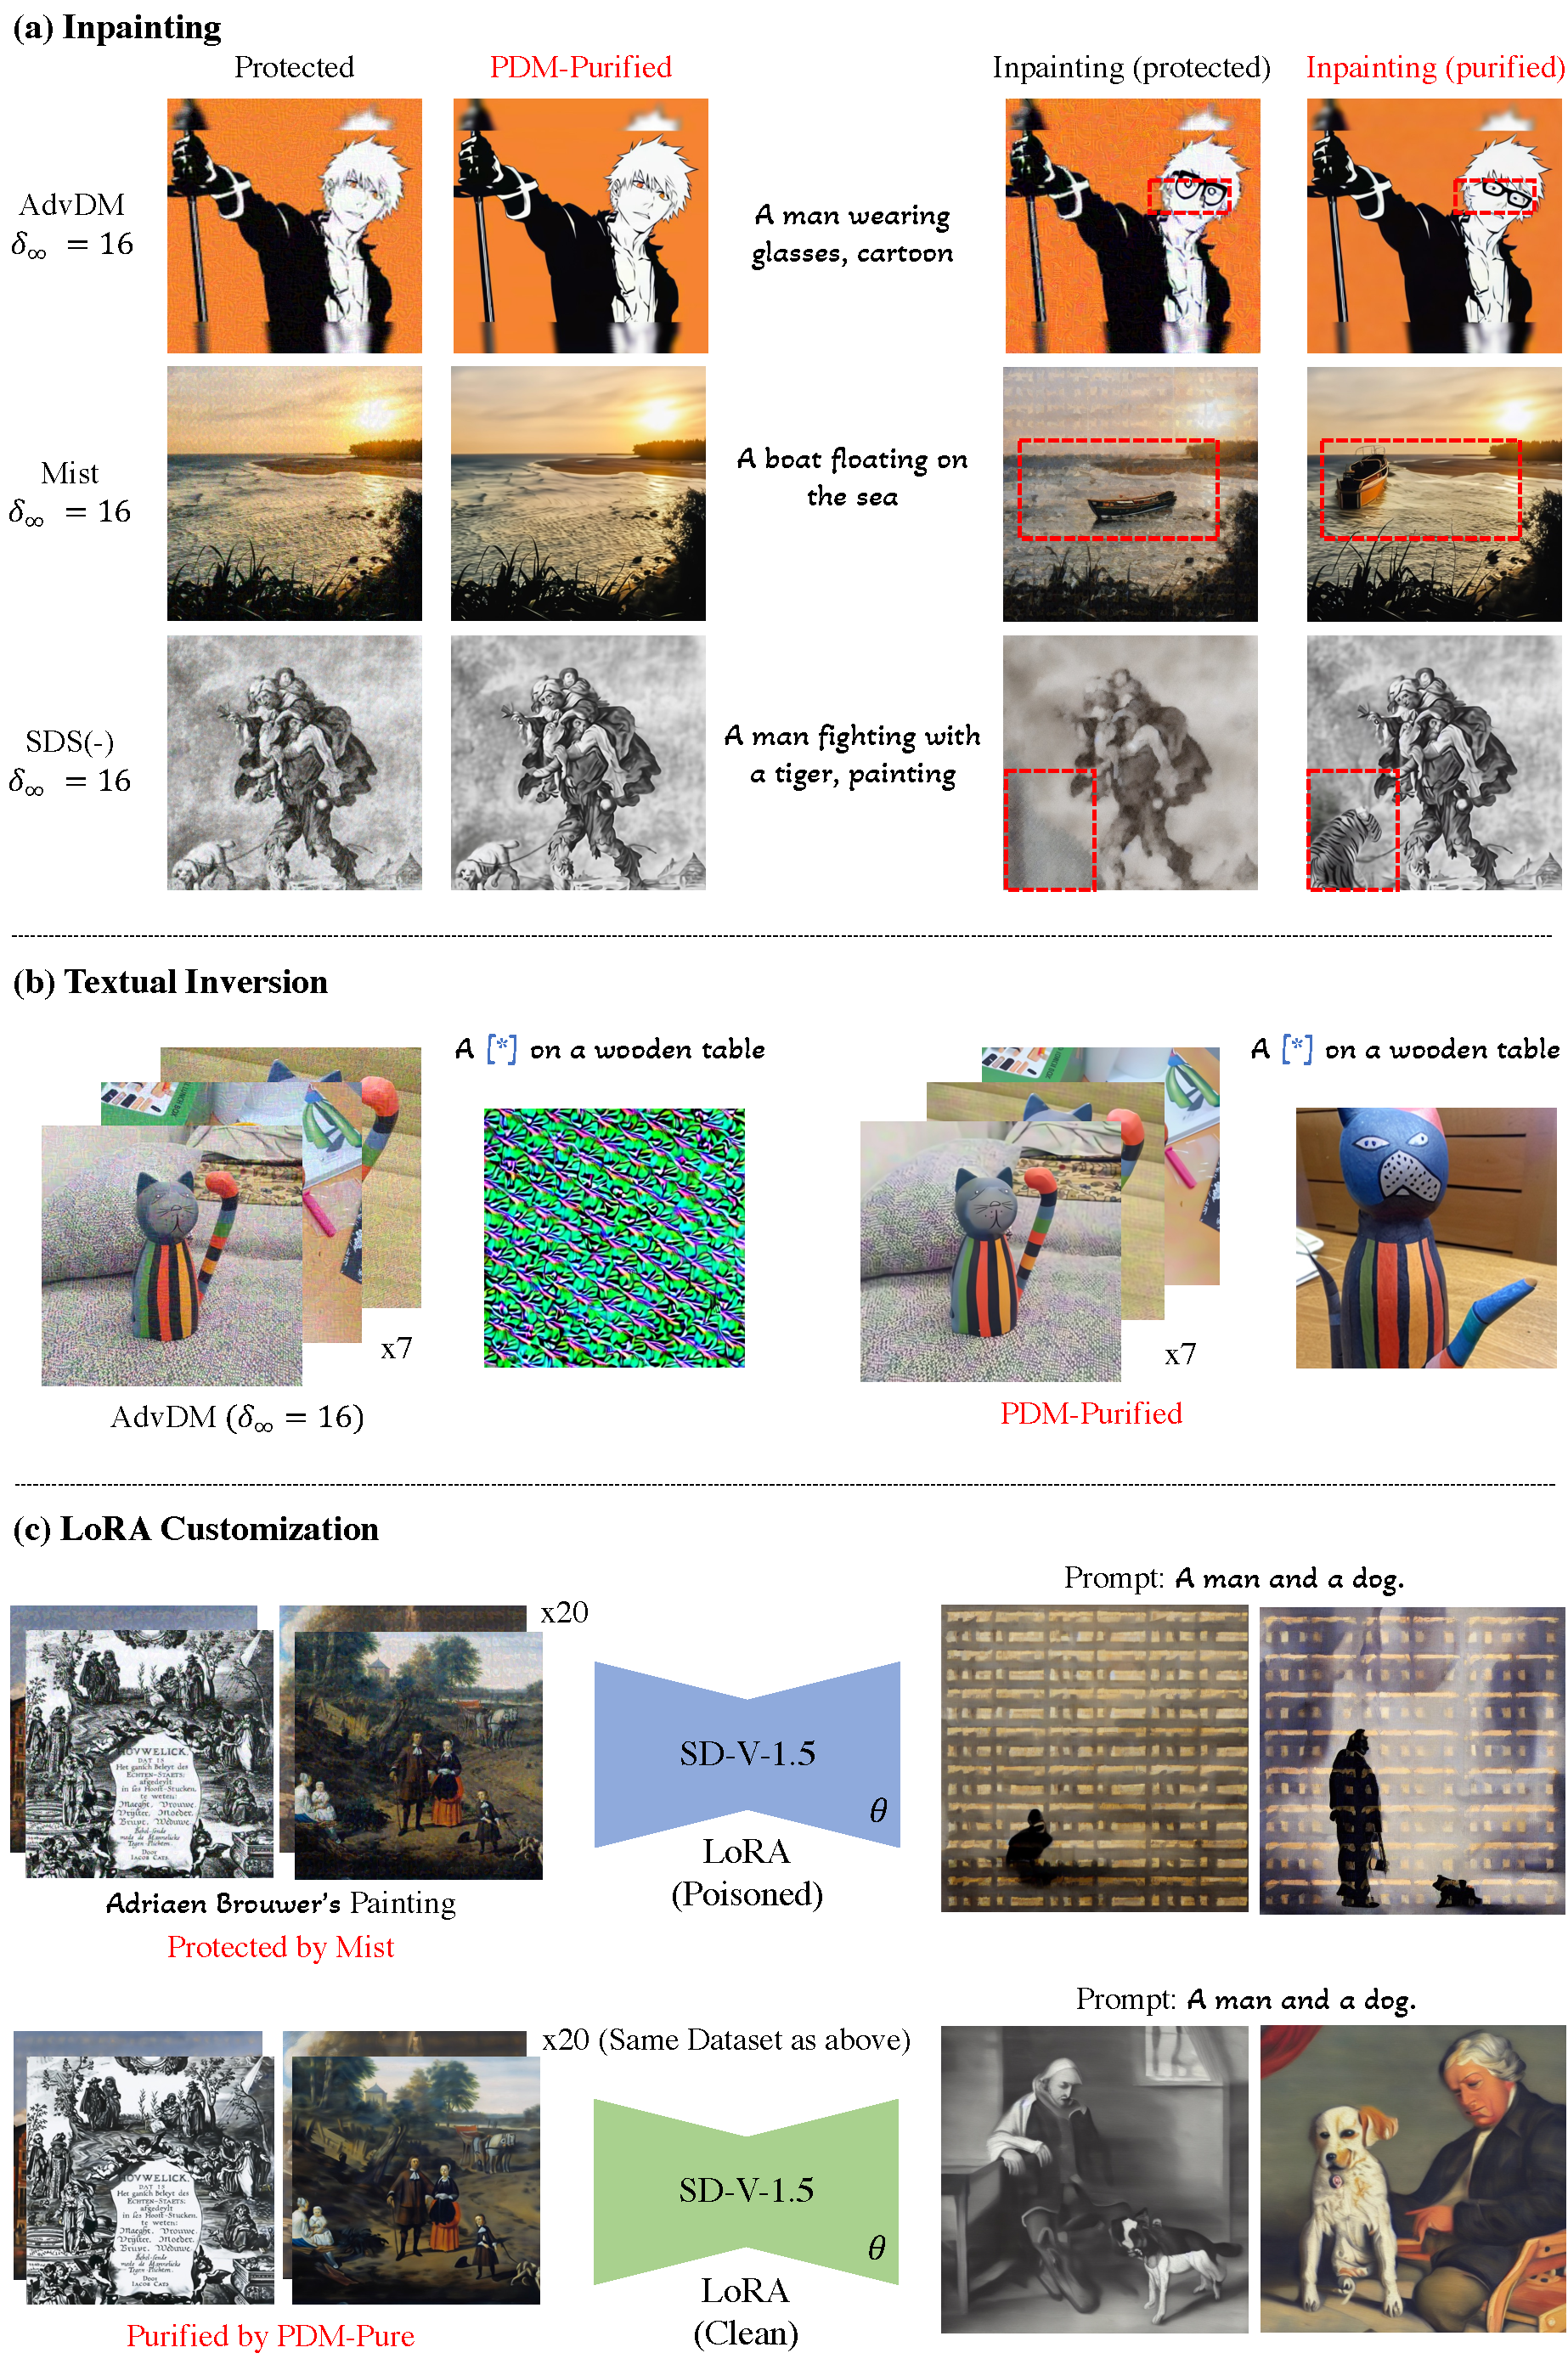
\includegraphics[width=0.99\linewidth]{images/lora.pdf}
  \vspace{-5pt}
  \caption{
  \textbf{PDM-Pure makes the Protected Images no more Protected:} Here we show qualitative results of PDM-Pure on three scenarios where unauthorized editing may occur: (a) Inpainting, (b) Text-Inversion~\cite{textualinversion} and (c) LoRA customization~\cite{lora}. While the protected images incur bad generation quality, the purified ones can fully bypass the protection.
  }
  % \caption{\textbf{Qualitative Results of PDM-Pure in Inpainting:} PDM-Pure can effectively remove the adversarial patterns in various protection methods, here we show image inpainting results on three typical protection methods: AdvDM~\cite{advdm}, Mist~\cite{liang2023mist} and SDS(-)~\cite{sdsattack} on Stable Diffusion V-1.5. We show results on quite strong attacks with budget $\delta_{\infty}=16/255$. We can see the figures are no more adversarial after PDM-Pure, resulting in much better inpainting results. (inpainting regions are indicated by the the bounding boxes; zoom in on screen for better observation)}

  \label{fig:purification_results}
\end{figure}
